% Options for packages loaded elsewhere
% Options for packages loaded elsewhere
\PassOptionsToPackage{unicode}{hyperref}
\PassOptionsToPackage{hyphens}{url}
\PassOptionsToPackage{dvipsnames,svgnames,x11names}{xcolor}
%
\documentclass[
  11pt,
]{article}
\usepackage{xcolor}
\usepackage[top=0.4in,bottom=0.45in,left=0.65in,right=0.65in,includehead,headheight=52pt,headsep=7pt,includefoot,footskip=24pt]{geometry}
\usepackage{amsmath,amssymb}
\setcounter{secnumdepth}{-\maxdimen} % remove section numbering
\usepackage{iftex}
\ifPDFTeX
  \usepackage[T1]{fontenc}
  \usepackage[utf8]{inputenc}
  \usepackage{textcomp} % provide euro and other symbols
\else % if luatex or xetex
  \usepackage{unicode-math} % this also loads fontspec
  \defaultfontfeatures{Scale=MatchLowercase}
  \defaultfontfeatures[\rmfamily]{Ligatures=TeX,Scale=1}
\fi
\usepackage{lmodern}
\ifPDFTeX\else
  % xetex/luatex font selection
\fi
% Use upquote if available, for straight quotes in verbatim environments
\IfFileExists{upquote.sty}{\usepackage{upquote}}{}
\IfFileExists{microtype.sty}{% use microtype if available
  \usepackage[]{microtype}
  \UseMicrotypeSet[protrusion]{basicmath} % disable protrusion for tt fonts
}{}
\makeatletter
\@ifundefined{KOMAClassName}{% if non-KOMA class
  \IfFileExists{parskip.sty}{%
    \usepackage{parskip}
  }{% else
    \setlength{\parindent}{0pt}
    \setlength{\parskip}{6pt plus 2pt minus 1pt}}
}{% if KOMA class
  \KOMAoptions{parskip=half}}
\makeatother
% Make \paragraph and \subparagraph free-standing
\makeatletter
\ifx\paragraph\undefined\else
  \let\oldparagraph\paragraph
  \renewcommand{\paragraph}{
    \@ifstar
      \xxxParagraphStar
      \xxxParagraphNoStar
  }
  \newcommand{\xxxParagraphStar}[1]{\oldparagraph*{#1}\mbox{}}
  \newcommand{\xxxParagraphNoStar}[1]{\oldparagraph{#1}\mbox{}}
\fi
\ifx\subparagraph\undefined\else
  \let\oldsubparagraph\subparagraph
  \renewcommand{\subparagraph}{
    \@ifstar
      \xxxSubParagraphStar
      \xxxSubParagraphNoStar
  }
  \newcommand{\xxxSubParagraphStar}[1]{\oldsubparagraph*{#1}\mbox{}}
  \newcommand{\xxxSubParagraphNoStar}[1]{\oldsubparagraph{#1}\mbox{}}
\fi
\makeatother


\usepackage{longtable,booktabs,array}
\newcounter{none} % for unnumbered tables
\usepackage{calc} % for calculating minipage widths
% Correct order of tables after \paragraph or \subparagraph
\usepackage{etoolbox}
\makeatletter
\patchcmd\longtable{\par}{\if@noskipsec\mbox{}\fi\par}{}{}
\makeatother
% Allow footnotes in longtable head/foot
\IfFileExists{footnotehyper.sty}{\usepackage{footnotehyper}}{\usepackage{footnote}}
\makesavenoteenv{longtable}
\usepackage{graphicx}
\makeatletter
\newsavebox\pandoc@box
\newcommand*\pandocbounded[1]{% scales image to fit in text height/width
  \sbox\pandoc@box{#1}%
  \Gscale@div\@tempa{\textheight}{\dimexpr\ht\pandoc@box+\dp\pandoc@box\relax}%
  \Gscale@div\@tempb{\linewidth}{\wd\pandoc@box}%
  \ifdim\@tempb\p@<\@tempa\p@\let\@tempa\@tempb\fi% select the smaller of both
  \ifdim\@tempa\p@<\p@\scalebox{\@tempa}{\usebox\pandoc@box}%
  \else\usebox{\pandoc@box}%
  \fi%
}
% Set default figure placement to htbp
\def\fps@figure{htbp}
\makeatother





\setlength{\emergencystretch}{3em} % prevent overfull lines

\providecommand{\tightlist}{%
  \setlength{\itemsep}{0pt}\setlength{\parskip}{0pt}}



 


% =====================================================================
%  _style.tex  ·  Design system for EIL research highlights (v4 layout)
%  Edit here to restyle ALL research highlights. Included via the .qmd YAML.
%  Matches the canonical single-column v4 template; the masthead and footer
%  are set per-document via fancyhdr in each .qmd's include-in-header.
% =====================================================================

% ---- Colours (exact hex) --------------------------------------------
\definecolor{ink}{HTML}{1D2620}        % headings, title, section heads, rule
\definecolor{body}{HTML}{33352C}       % main body paragraphs
\definecolor{accentred}{HTML}{641111}  % RESEARCH HIGHLIGHT label, links, fig title
\definecolor{boxred}{HTML}{8C2826}     % Bottom Line box fill
\definecolor{boxtext}{HTML}{EEF1EA}    % Bottom Line body text (off-white)
\definecolor{muted}{HTML}{50534A}      % figure source line
\definecolor{cite}{HTML}{6E6D61}       % citation line
\definecolor{faint}{HTML}{9A978A}      % footer
\definecolor{warmrule}{HTML}{D8D2C2}   % thin warm-grey dividers
\definecolor{paper}{HTML}{FAF8F1}      % warm page background

% \pagecolor{paper}                    % uncomment for warm off-white background

% ---- Fonts (Source Sans 3 / Source Serif 4) -------------------------
\usepackage[T1]{fontenc}
\usepackage[default]{sourcesanspro}
\usepackage{sourceserifpro}
\renewcommand{\familydefault}{\sfdefault}

% ---- Page -----------------------------------------------------------
\pagestyle{empty}
\setlength{\parindent}{0pt}
\setlength{\parskip}{2pt}
% Default body size/colour. The v4 .qmd overrides this to 10.5/13.5pt.
\AtBeginDocument{\color{body}\fontsize{9.4pt}{13.6pt}\selectfont}

% ---- Packages -------------------------------------------------------
\usepackage{microtype}
\usepackage{soul}
\setul{2pt}{.5pt}
\usepackage{tcolorbox}
\tcbuselibrary{skins}
\usepackage[colorlinks=true, urlcolor=accentred, linkcolor=accentred, pdfborder={0 0 0}]{hyperref}

% =====================================================================
%  MACROS
% =====================================================================

% --- Title + citation (citation has a thin warm divider beneath) ------
\newcommand{\brieftitle}[1]{%
  {\color{ink}\fontsize{18pt}{19.5pt}\selectfont\bfseries\textls[-12]{#1}\par}\vspace{3pt}}
\newcommand{\briefcitation}[1]{%
  {\color{cite}\fontsize{9.4pt}{12pt}\selectfont #1\par}\vspace{3pt}%
  \noindent\textcolor{warmrule}{\rule{\linewidth}{0.7pt}}}

% --- Section heads (uppercase, ink) ----------------------------------
\newcommand{\sectionhead}[1]{%
  \vspace{2pt}{\color{ink}\bfseries\fontsize{9.75pt}{12pt}\selectfont
  \textls[20]{\MakeUppercase{#1}}\par}\vspace{1pt}}

% --- Sub-heads (small uppercase) — Takeaway subheads -----------------
% The v4 .qmd overrides this to the brand maroon via \renewcommand.
\newcommand{\subhead}[1]{%
  {\color{ink}\bfseries\fontsize{8.25pt}{10pt}\selectfont
  \textls[50]{\MakeUppercase{#1}}\par}\vspace{2pt}}

% --- Figure title + source line --------------------------------------
\newcommand{\figtitle}[2]{%
  {\bfseries\color{accentred}\fontsize{7.1pt}{9pt}\selectfont\textls[40]{\MakeUppercase{#1}}}\par%
  {\color{muted}\fontsize{7.1pt}{9pt}\selectfont #2}\par\vspace{4pt}}

% =====================================================================
%  COLOURED BOXES
% =====================================================================

% --- Bottom Line box (border-radius 6px -> arc=4pt) ------------------
\newtcolorbox{bottomline}{%
  enhanced, arc=4pt, outer arc=4pt, boxrule=0pt,
  colback=boxred, coltext=boxtext,
  left=7pt, right=7pt, top=7pt, bottom=7pt,
  before upper={\fontsize{9.4pt}{13.6pt}\selectfont}}
% --- Running masthead + footer (logo, label, rule, page number) ---
\usepackage{fancyhdr}
\renewcommand{\headrulewidth}{0pt}
\renewcommand{\footrulewidth}{0pt}
\fancypagestyle{brief}{%
  \fancyhf{}%
  \fancyhead[L]{%
    \begin{minipage}[c]{0.62\textwidth}\raggedright\color{ink}
\includegraphics[height=0.45in]{../../../../formats/logos/eil-logo-maroon.png}\end{minipage}\hfill%
    \begin{minipage}[c]{0.36\textwidth}\raggedleft\fontsize{8.25pt}{10pt}\selectfont\bfseries\color{accentred}\textls[200]{\MakeUppercase{Research Highlight}}\end{minipage}%
    \par\vspace{2pt}%
    \noindent\textcolor{ink}{\rule{\textwidth}{2.2pt}}%
  }%
  \fancyfoot[C]{%
    \color{warmrule}\rule{\textwidth}{0.7pt}\par\vspace{3pt}%
    \hbox to\textwidth{%
      \color{faint}\fontsize{7.4pt}{9pt}\selectfont
      For full paper:\hspace{0.4em}\href{https://doi.org/10.1002/pam.70056}{\color{faint}\underline{\textls[40]{doi.org/10.1002/pam.70056}}}%
      \hfill
      Page \thepage%
    }%
  }%
}
\pagestyle{brief}
% Takeaways subheads in the brand maroon (logo / Research Highlight)
\renewcommand{\subhead}[1]{%
  {\color{accentred}\bfseries\fontsize{8.25pt}{10pt}\selectfont
  \textls[50]{\MakeUppercase{#1}}\par}\vspace{2pt}}
\makeatletter
\@ifpackageloaded{caption}{}{\usepackage{caption}}
\AtBeginDocument{%
\ifdefined\contentsname
  \renewcommand*\contentsname{Table of contents}
\else
  \newcommand\contentsname{Table of contents}
\fi
\ifdefined\listfigurename
  \renewcommand*\listfigurename{List of Figures}
\else
  \newcommand\listfigurename{List of Figures}
\fi
\ifdefined\listtablename
  \renewcommand*\listtablename{List of Tables}
\else
  \newcommand\listtablename{List of Tables}
\fi
\ifdefined\figurename
  \renewcommand*\figurename{Figure}
\else
  \newcommand\figurename{Figure}
\fi
\ifdefined\tablename
  \renewcommand*\tablename{Table}
\else
  \newcommand\tablename{Table}
\fi
}
\@ifpackageloaded{float}{}{\usepackage{float}}
\floatstyle{ruled}
\@ifundefined{c@chapter}{\newfloat{codelisting}{h}{lop}}{\newfloat{codelisting}{h}{lop}[chapter]}
\floatname{codelisting}{Listing}
\newcommand*\listoflistings{\listof{codelisting}{List of Listings}}
\makeatother
\makeatletter
\makeatother
\makeatletter
\@ifpackageloaded{caption}{}{\usepackage{caption}}
\@ifpackageloaded{subcaption}{}{\usepackage{subcaption}}
\makeatother
\usepackage{bookmark}
\IfFileExists{xurl.sty}{\usepackage{xurl}}{} % add URL line breaks if available
\urlstyle{same}
\hypersetup{
  colorlinks=true,
  linkcolor={blue},
  filecolor={Maroon},
  citecolor={Blue},
  urlcolor={Blue},
  pdfcreator={LaTeX via pandoc}}


\author{}
\date{}
\begin{document}


% ---------------------------------------------------------------------
% TITLE + CITATION  (masthead now repeats in the page header)
% ---------------------------------------------------------------------
\brieftitle{EPA Compliance Workshops Don't Reduce Violations}
\briefcitation{Lessons from ``The effect of compliance assistance on pollution discharges and violations of environmental regulations'' by Paul J. Ferraro \& Jay P. Shimshack in \textit{Journal of Policy Analysis and Management}, 2026.}

\vspace{-2pt}

% override body font size for this document
\fontsize{10.5pt}{13.5pt}\selectfont

% ---------------------------------------------------------------------
% BOTTOM LINE
% ---------------------------------------------------------------------
\begin{bottomline}
{\fontsize{11pt}{15pt}\selectfont
\textbf{Offering polluters free help to follow the rules doesn't make them more likely to follow them.} New research studying hundreds of facilities that were offered free compliance workshops found the workshops didn't reduce violations.
}
\end{bottomline}

\vspace{6pt}

% ---------------------------------------------------------------------
% BACKGROUND
% ---------------------------------------------------------------------
\sectionhead{Background}
\noindent Environmental enforcement in the U.S. has long centered on penalties: inspect facilities, catch violations, and levy fines. \textbf{Compliance assistance} takes a different approach: \textbf{regulators help facilities follow the rules in the first place, through free workshops, guidance, and technical support.} The premise is that many violations stem from confusion or limited expertise rather than deliberate corner-cutting. While compliance assistance is becoming increasingly favored by the Environmental Protection Agency (EPA) over penalties, \textbf{whether it's actually effective has rarely been tested}.

\noindent In a new study, researchers set out to better understand how effective compliance assistance actually is, using data on hundreds of wastewater treatment facilities regulated by the Ohio EPA. Facilities that had recently been cited for violations were invited to participate in compliance workshops, which were rolled out over several months. Those that volunteered to attend received free training on how to comply with the Clean Water Act. The researchers then compared the facilities that attended the workshops against those that had not yet been trained, tracking whether violations fell after the workshops.

\vspace{6pt}

% ---------------------------------------------------------------------
% WHAT THE STUDY FOUND
% ---------------------------------------------------------------------
\sectionhead{What the study found}
% ---------------------------------------------------------------------
% FIGURE — event study: effect on violations by month around training
% ---------------------------------------------------------------------
\begin{center}
\begin{minipage}{0.82\linewidth}
\figtitle{The workshops' effect on violations, month by month}{Source: Ferraro \& Shimshack (2026).}
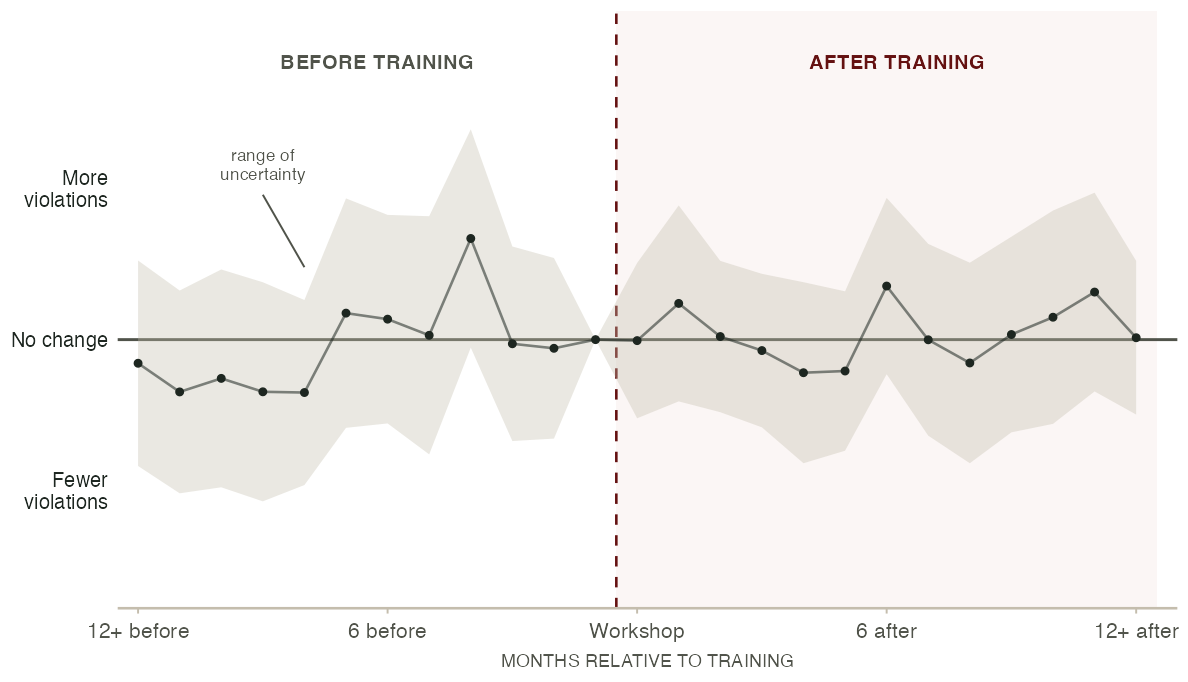
\includegraphics[width=\linewidth]{../../data-viz/figures/fig2-did.png}
\par\vspace{3pt}
{\color{faint}\fontsize{7.1pt}{9.5pt}\selectfont \textit{Note:} Each point compares violations at trained facilities against facilities not yet trained, month by month around training (month 0). After training, an effect from the workshops would show up as the line moving away from zero; instead it stays flat, and the shaded band of statistical uncertainty always includes ``no change.'' The workshops had no detectable effect.\par}
\end{minipage}
\end{center}

\vspace{6pt}

\newpage

\noindent Evaluating whether a policy works is difficult: researchers can't see what the facilities would have done with and without the policy. Two things make this policy hard to evaluate. First, the workshops were voluntary. This means that comparing trained and untrained facilities might not work --- what if facilities that signed up were more motivated to reduce violations than those that didn't, regardless of the workshops? That could conflate two different causes of violation reduction. Second, violations were falling across the board in these years, so a simple before-and-after comparison would credit the workshops with a broader decline they hadn't caused. 

\noindent The researchers got around both by comparing facilities trained early against ones that had \emph{also} signed up but not yet been trained. Those facilities were just as motivated, having volunteered too, and they were measured over the same period, so the across-the-board decline in violations showed up in both. The staggered rollout, spread over several months, is what made those not-yet-trained facilities available as a comparison group. Of course, the not-yet-trained facilities are only a fair stand-in if they really would have followed the same path, and that's something researchers have to assume.

\noindent The two groups declined almost identically. Violations at trained facilities fell by about as much as at facilities still waiting to be trained, and no additional drop appeared once a facility had been through a workshop. \textbf{Trained facilities were no less likely to violate than facilities that had not yet been trained.}

\vspace{8pt}

% ---------------------------------------------------------------------
% TAKEAWAY
% ---------------------------------------------------------------------
\sectionhead{Takeaways}
\subhead{The limits of assistance}
\noindent If free guidance has no effect on violations, the obstacles to compliance likely lie in the costs, capacity, or incentives that shape how facilities operate day to day, not a lack of knowledge. That matters for a program that the EPA is considering expanding. As agencies increasingly turn to assistance in place of enforcement, this study suggests compliance assistance should be treated as a hypothesis to be tested, not a solution to be assumed. \textbf{A widely adopted tool still has to prove it works.}

\vspace{5pt}
\subhead{Proof before scale}
\noindent The workshops are a case study in how easily a policy can appear to work. Promising before-and-after comparisons can capture trends that were already in motion, but a careful comparison can separate a real effect from a coincidence. Before a promising program is expanded to new places, its apparent success should have to survive that kind of scrutiny. \textbf{Good evidence is what separates a policy that works from one that only looks like it does.}




\end{document}
